\chapter{Frameworks}
\section{Introduction to Machine Learning}

Machine learning is a powerful tool that can be used to identify patterns in complex datasets. In the context of particle physics, machine learning algorithms can be used to detect signals from background noise in large datasets generated by detectors. In particular, for the detection of IBD signals from background, machine learning algorithms can be used to identify patterns in the data that are indicative of an IBD event, and to distinguish these signals from the background noise explained above. Moreover, one advantage of machine learning for particle physics is that it can handle large amounts of data and identify subtle patterns that may be difficult for humans to detect.
\\


\subsection{Supervised Learning}

Supervised learning is a machine learning technique in which the algorithm is trained on a labelled dataset, where the input data is accompanied by the correct output. The goal of the algorithm is to learn a function that can map input data to output data. Some examples of supervised learning algorithms include linear regression, logistic regression, decision trees, and support vector machines. Despite the complexity and diversity of these methods, it's more advantageous to illustrate the profound concepts of machine learning through a simple machine learning algorithm, such as linear regression. 

\subsection{Linear Regression}
Linear regression is a type of supervised learning algorithm used in machine learning for predictive analysis. It is used to model the relationship between a dependent variable, called the target, and one or more independent variables, called the features.
\\
The basic idea behind linear regression is to find the best-fitting hyper-plane that describes the relationship between the independent and dependent variables. The equation for the hyper-plane can be written as:

\begin{equation}
	y = w_0 + w_1 x_1 + w_2 x_2 + ... + w_n x_n 
\end{equation}
 where 
\begin{itemize}
	\item $y$ is the dependent variable
	\item $x_1, x_2, ..., x_p$ are the independent variables
	\item $w_0, w_1, w_2, ..., w_n$ are the coefficients or parameters of the model
\end{itemize}

In order to determine the values of the coefficients $w_0, w_1, w_2, ..., w_n$, a common approach is to minimize a loss function, which measures the difference between the predicted values of the dependent variable and the actual values. The most commonly used loss function in linear regression is the mean squared error (MSE) function, which is defined as:

\begin{equation}
	L(w_0, w_1, w_2, ..., w_n) = \frac{1}{n} \sum_{i=1}^{n} (y_i - \hat{y_i})^2
\end{equation}

where $n$ is the number of observations, $y_i$ is the actual value of the dependent variable for the $i$-th observation, and $\hat{y_i}$ is the predicted value of the dependent variable for the $i$-th observation.


The objective of linear regression is to determine the optimal values of coefficients $w_0, w_1, w_2, ..., w_n$ that minimize a predefined loss function $L(w_0, w_1, w_2, ..., w_n)$. One commonly employed method to accomplish this is the gradient descent algorithm.\\


Gradient descent is an iterative optimization technique for finding the local minimum of a function. To apply gradient descent in the context of a linear regression problem, we initialize the coefficients with random values and then iteratively update these values in the direction that decreases the loss function the most.

Mathematically, the update rule for each coefficient is:

\begin{equation}
	w_j^{(new)} = w_j^{(old)} - \alpha \frac{\partial L}{\partial w_j}
\end{equation}


where $w_j^{(new)}$ and $w_j^{(old)}$ are the new and old values of the j-th coefficient, $\alpha$ is the learning rate, and $\frac{\partial L}{\partial w_j}$ is the partial derivative of the loss function with respect to the j-th coefficient. The learning rate $\alpha$ determines the size of the steps we take towards the minimum.

Once we reach a point where the loss function no longer decreases (or decreases very slowly), we stop the iteration and accept the current values of coefficients as the solution.
\\

However, it is important to note that linear regression, and also other machine learning alghoritms can suffer from overfitting or underfitting. Overfitting occurs when the model is too complex and captures noise in the data, while underfitting occurs when the model is too simple and fails to capture the underlying patterns in the data. To prevent overfitting or underfitting, regularization techniques can be used.

\newpage

\section{Binary Classification}

\section{Decision Tree}
Decision trees are a cornerstone of machine learning algorithms, providing a robust model that segments the feature space into various non-overlapping regions. The model is capable of conducting both regression and classification tasks, creating rules from the available features to predict the value of a target variable.

Mathematically, we can represent the decision tree model as follows. Given a dataset $D$ containing $n$ instances, where each instance $i$ is an input-output pair $(x_i, y_i)$ with $x_i$ belonging to the input space $X$ and $y_i$ to the output space $Y$. The decision tree maps an instance $x_i$ to an output $y_i$ through a series of binary tests:

 \begin{equation}
	y_i = f(x_i) = \sum_{j=1}^{J} c_j I(x_i \in R_j)
\end{equation}


where $f(x_i)$ is the decision tree, $R_j$ are the disjoint regions of the feature space, $I()$ is the indicator function, and $c_j$ is the predicted value in region $j$.

To grow a decision tree, we start at the root and recursively split the data based on the feature that maximizes the reduction of a chosen impurity measure. Common measures include entropy and the Gini index, calculated as follows:

Entropy: $Entropy(S) = - \sum_{i=1}^{c} p_i \log_2(p_i)$

Gini Impurity: $Gini(S) = 1 - \sum_{i=1}^{c} (p_i)^2$

\subsection{Boosted Decision Trees}
 
Boosting is a meta-algorithm in machine learning, developed to convert weak learners into a strong predictive model. Boosted decision trees are an implementation of this concept, often leading to significantly improved model performance.

Boosted decision trees work on the principle of fitting the boosting model $F(x)$ by minimizing the loss function $L(y, F(x))$ over the training data. This is typically done in a stage-wise fashion. Given the current model $F_m(x)$, we fit a weak learner (a small decision tree, $h(x)$) to the negative gradient of the loss function, evaluated with the current model and updated as:

$F_{m+1}(x) = F_{m}(x) + \alpha h(x)$

where $\alpha$ is a constant, often set via line search to minimize the loss function.

Gradient Boosting and AdaBoost are two common methods. XGBoost, or eXtreme Gradient Boosting, stands as a notable Gradient Boosting variant. It introduces regularization parameters to prevent overfitting, handles missing values, and utilizes both parallelized and distributed computing, making it suitable for large-scale problems.

\begin{figure}[h!]
	\centering
	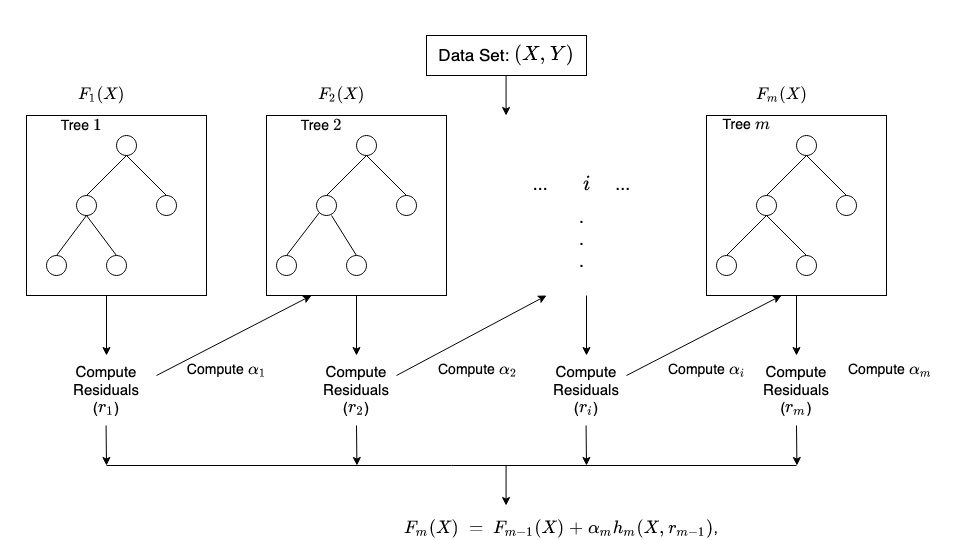
\includegraphics[width=0.8\linewidth]{Images/XGBoost}
	\caption{}%https://docs.aws.amazon.com/it_it/sagemaker/latest/dg/xgboost-HowItWorks.html}
	\label{fig:xgboost}
\end{figure}


\section{Neural Networks}